\documentclass[main.tex]{subfiles}

\graphicspath{{./img}}
\begin{document}
\section{Intelligent Transport Systems}\label{sec-its}

Intelligent transport systems describe an initiative to utilize modern technology 
in order to optimize and increase efficiency of processes common to the domain of transportation. 
This usually involves enabling different actors in the transportation system to communicate 
with each other and share available information (much like multi-agent systems). With the 
availability of shared information, complex, data-driven systems can be built utilizing 
state-of-the-art tech concepts like machine learning, computer vision and IoT, while
integrating road users to improve street protection and increase traffic efficiency and stability.
İt also address environmental issues via controlling traffic to prevent congestion or lessen
their adverse effects. 

When looked at these solution from a systemic point of view, they can 
be, in less or more ways, resemble multi-agent systems. This section will be focused more on 
the \emph{inductive} part of research, examining various existing ITS solutions and trying 
to recognize their agent-based characteristics and principles, to determine possible application 
of MAS for simulation of ITS systems, whether suitable application for agent-based modelling of 
ITS is feasible. The insights gained by reviewing current state of ITS will 
serve as a base for further sections, where considerations regarding model framework design and 
its validation will be discussed. 

\begin{figure}[htbp]
    \centering
    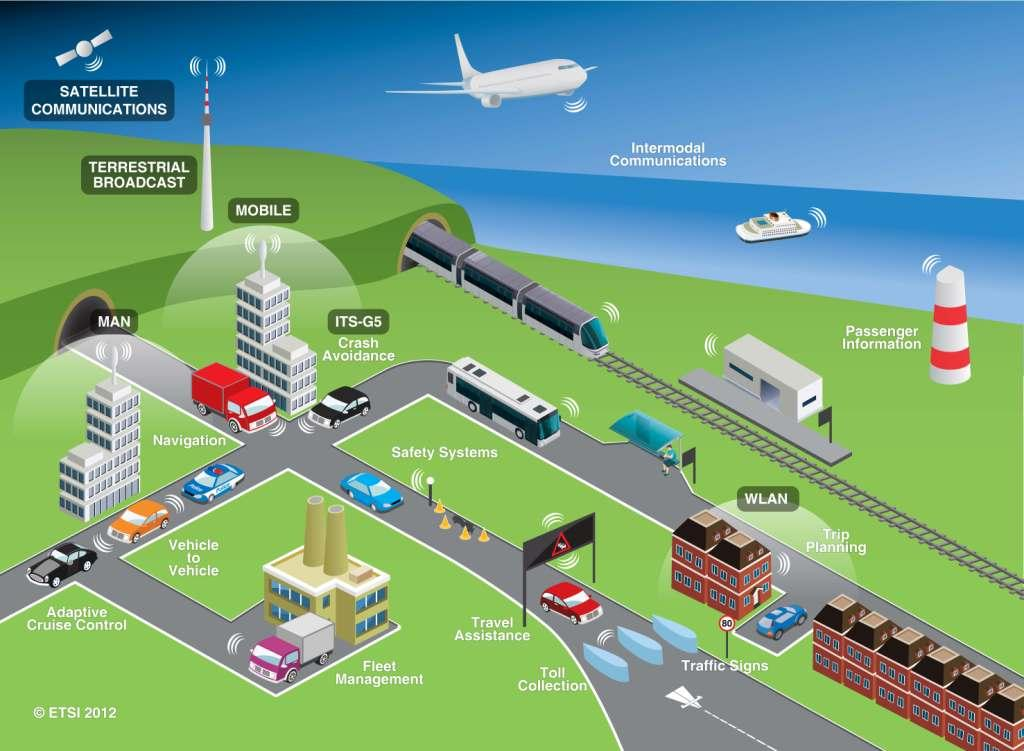
\includegraphics[width=.8\textwidth]{ITS-schema.jpg}
    \caption{Illustration of an ITS topology \cite{ETSI}}
    \label{its-map}
\end{figure}

ITS can provide itself most useful in the following aspects of transportation: 
\emph{Mobility}, \emph{Safety}, \emph{Environment} \cite{Lishchenko2021}. To provide an example, regarding mobility, 
one of the most common systems is routing and navigation for road users. These systems can 
factor in time, distance and even emissions when providing route guidance \cite{Firmin2006}. This leads to 
increased performance of road networks. Regarding safety, one can mention emergency management
systems like E-Call, which provides automated post-crash assistance by contacting emergency
services as soon as an incident happens. In terms of the environment, 
ITS allows for demand management through \emph{electronic fee collection}, which makes flexible 
charging for road usage possible, based on vehicle type and emissions category \cite{Commision2022}.
Another, more general example of emissions reduction of ITS is through reducing congestions, as road vehicle 
emissions have proven to be a significant environmental factor especially because they produce emissions 
in highly human-populated areas, exposing large number of population to serious health risks. In a study conducted by the Harvard
School of Public Health, air pollution from traffic congestion in 83 of the USA's largest urban
areas contributes to more than 2,200 premature deaths annually, costing the health care system at
least \$18 billion \cite{Levy2011}.

\subsection{IVS-based research}

Using virtual simulation tools to research and evaluate impacts of new and existing ITS 
is a great tool, as it can greatly reduce the overall cost of development, achieved by faster, 
and flexible development in virtual space allowing for frequent, iterative evaluation of features.

It is important to say that ITS solutions vary in terms of \emph{driver engagement}. Because
the primary use-case of interactive vehicle simulator is to research driver behaviour, the 
scope of the current state of ITS will be focused on ITS solutions that integrate automotive 
transport and have some form of driver engagement, favouring solutions that have a large degree 
of interaction with the driver.

\begin{figure}[htbp]
    \centering
    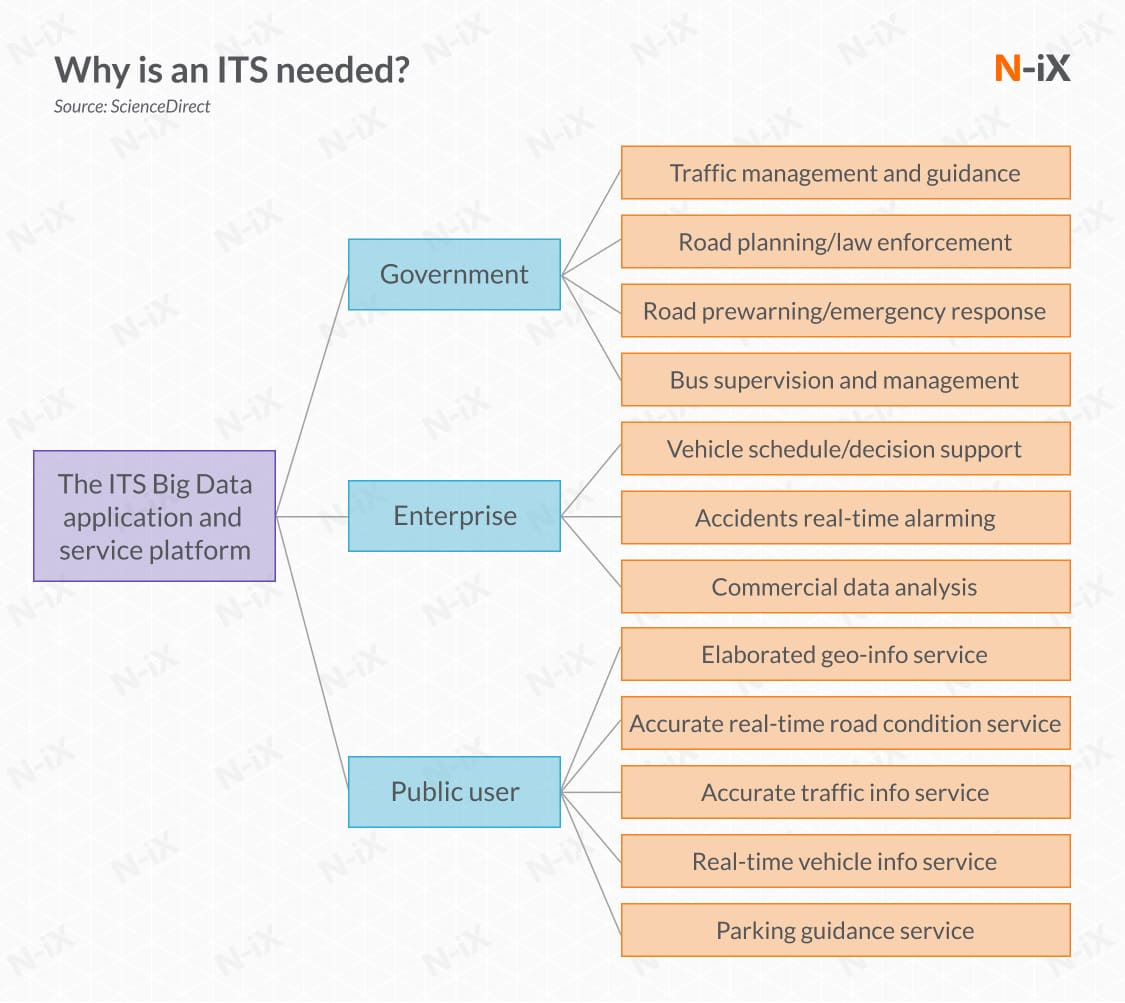
\includegraphics[width=.8\textwidth]{why is ITS needed.jpg}
    \caption{Reasons for ITS usage \cite{Lishchenko2021}}
    \label{whyITS}
\end{figure}

As per figure (\ref{whyITS}), there are ITS use-cases with high degree of driver interaction (determined 
by trivial logic). The observed use-cases with high driver engagement were determined as such:

\begin{itemize}
    \itemspacing{.7}
    \item Geo-info service
    \item Real-time road condition service 
    \item Accurate traffic-info service 
    \item Real-time vehicle info service 
    \item Parking guidance service
\end{itemize}

These use-cases should be considered when modelling the ITS simulation framework in the practical part of the 
thesis to make these ITS use-cases easy to deploy and simulate.

\subsection{Intelligence distribution} \label{mas-compatibility}

It is important to acknowledge whether the underlying system control is centrally governed 
or whether the intelligence is distributed across multiple actors, where individual 
components of the system are able to act semi- or fully independently.
Such self-imposed reasoning is important to consider, because the way ITS solutions 
with centralized or distributed intelligence are designed can be fundamentally different 
and this, different system models are optimal to use when simulating a particular ITS. 
Intelligent transport systems are, by nature, systems combining several actors together to
achieve a common goal. This, however, doesn't mean that it is optimal to model \emph{every} ITS 
as a multi-agent system. 

Historically speaking, ITSs that were
developed and proved helpful for optimizing traffic were \emph{centralized} \cite{Corman2010}, meaning there is a
single, central component in charge of the decision-making logic, organizing other units/actors within the
system, while interacting with the drivers in the traffic as external actors. The main
advantage of these systems is that they are less complex, therefore it is easier to develop a resilient and
safe product. The main drawback of this method is that they are heavily affected by the size
of instances, increasing the complexity and often result in exceedingly large computation time,
making the solution sub-optimal \cite{Corman2010}. 

As with the \emph{distributed} systems, the main problem is systematically distributed to
individual agents solving a sub-problem and cooperating to achieve optimal and predictable
results, such distributed intelligence is often modelled using \emph{Multi-agent Systems}. 
This topic will be further discussed in chapter (\ref{sec-mas}). Distributed systems can be used to
solve traffic optimization problems on a larger scale. These systems have seen larger usage
especially in the recent times, as newly produced vehicles are equipped with powerful computers
that can be used to transfer the computational burden from the core computer in centralized
systems, thanks to the state-of-art communication protocols like DSRC and ITS 5G, which enable
low-latency direct communication between vehicles. 

The one example of ITS where implementations have been carried out in both centralized and 
decentralized principles numerous times is a \emph{Network traffic control}. The goal of this 
system is to use knowledge about the traffic on the network to control traffic lights and other 
active control elements to optimize traffic flow and decrease travel time. In a recent research 
reviewing signal timing optimization approaches, centralized and distributed network traffic
control systems were compared. The conclusion was that although the centralized system was able
to achieve better performance higher global efficiency, the decentralized solution required
significantly less computation time (40 \% in their experiment case) \cite{Chow2019}.

Other decentralized systems that are more exposed to the user (i.e. driver) include the 
\emph{Adaptive Cruise Control} (ACC). ACC extends the usual cruise control systems 
that maintain vehicle speed by adapting to speed of the vehicle in front, if there is any. In fact, 
recent development has lead to a further improvement, making ACC a cooperative system (CACC) that 
enables vehicles to adopt a \emph{driving strategy} by communicating with the infrastructure (V2I 
communication).

\subsubsection{Current research}\label{sec-research}

Secondly, it is important to choose a system that is time-relevant and would bring benefit to
current as well as future IVS and HMI research activities. Therefore, the third quality for choosing 
an ITS to implement would be one that is still subject to research and current trends in 
the ITS industry and explore state-of-the-art ITS. In order to determine which ITSs are relevant, 
it is important to review ongoing project of governmental bodies and their strategies and also
current trends in automotive ITS research activities.

In Europe, there are initiatives to centralize decision making and ITS deployment on the scale of 
the European continent. The reason behind this initiative is quite clear - to enable Europe-wide 
interoperability between deployed ITS and ITS-enabled vehicles. It is without a question that 
such organization would closely work with the industry, helping to create conditions for novel 
ITS technologies to be deployed.

\paragraph{ERTICO}

One such European organization is the \emph{European Road Transport Telematics
Implementation Coordination (ERTICO)} - a public-private partnership organization
with close to 120~members, connecting 8 different sectors in the ITS Community, including
service providers, suppliers, traffic and transport industry, research institutions and
universities, public authorities, user organizations, connectivity industry as well as
vehicle manufacturers \cite{ertico}.

As of now, ERTICO's activities focus on the following areas:

\term{Connected Cooperative \& Automated Mobility}
As the computational power of newly-produced vehicles is increasing dramatically with every 
new generation, as well as the number of sensor data, ERTICO states their focus is on utilizing 
the large amounts of real-life data to deepen the machine learning models, as well as building 
an infrastructure that will allow handling this data. C-ITS (Cooperative Intelligent Transport
Systems) is also mentioned, whose principles are being put into practice by several projects, 
namely European Truck Platooning (ETPC), Advanced map-enhanced driver assistance systems (ADASIS) and 
more. ERTICO's main contribution is to facilitate creation of ITS ecosystem by following a
multidisciplinary approach involving all relevant transport stakeholder sectors.

\term{Clean \& Eco Mobility}
As has been already mentioned, smart mobility innovations make a major contribution towards 
reducing the impact of transport-induced pollution, which has got a non-negligible contribution to 
global greenhouse gas emissions production \cite{Ritchie2020}. Below are the four main
objectives in the are of Clean \& Eco-Mobility. 

\begin{itemize}
    \setlength\itemsep{-10pt}
    \item Develop a common approach to the evaluation of ITS deployment as a tool for emissions reduction
    \item Contribute to smart mobility solutions being recognized as a tool for reducing emissions
    \item Achieve interoperability of electro-mobility
    \item Contribute to creating an ICT network with seamless and interoperable electro-mobility services
\end{itemize}

\term{Urban Mobility}
Another focus of ERTICO is Urban Mobility, where the main goal is to provide "Mobility as a Service" (MaaS), 
which is a system that could decrease congestions and provide low-carbon and -emission multi-modal transport 
solutions.  

\term{Transport \& Logistics}
ERTICO states that the current European world of transport and logistics is too fragmented, so an effort to 
develop solution for connecting logistics information system would optimize cargo flows and facilitate supply 
chain management. 

In conclusion, the ERTICO organization helps to reduce time to market of innovative,
state-of-the-art technologies, increasing inter-operability between individual ITS by promoting
an open framework for integration and deployment of intelligent transport services. 

As described above, there are potential systems that are yet to be fully implemented and
deployed for consumer use. 

\paragraph{Cooperative ITS}

Cooperative Intelligent Transport Systems (C-ITS) refers to transport systems, where ITS 
subsystems (personal, vehicle, roadside and central) cooperate. This
enables and provides an ITS service that offers better quality and an enhanced service level,
compared to the same ITS service provided by only one of the ITS sub-systems \cite{2022}.
An example of the concept of the technology can be seen in the figure (\ref{c-its}) below. 

\begin{figure}[htbp]
    \centering
    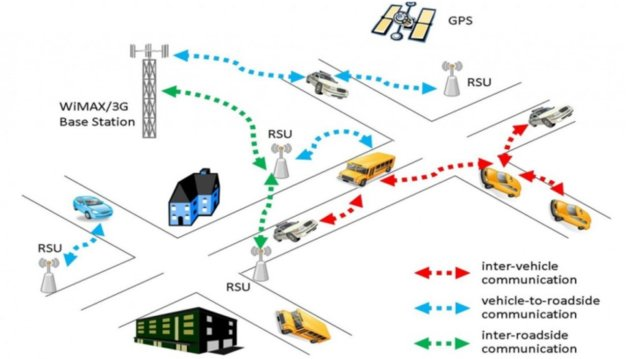
\includegraphics[width=.8\textwidth]{c-its.jpg}
    \caption{Example schematic of C-ITS scenario}
    \label{c-its}
\end{figure}

The concept of C-ITS was developed by the European Commission, representatives of industry and 
authorities in the European Union. In 2016, it was agreed on a coordinated establishment of intelligent
transport systems in Europe. It is considered to be one of the various tools to facilitate achieving 
the \emph{vision zero}, which is a project that aims to mitigate all fatalities involving road 
transport.

The European Commission outlined its plan for the coordinated deployment of C-ITS in Europe in
its communication 'A European strategy on Cooperative Intelligent Transport Systems', in which
it also states that the full-scale deployment of C-ITS services and C-ITS enabled vehicles is
expected to start in 2019.

The main feature of C-ITS is its distributed intelligence across vehicles and the infrastructure, 
which is a novel concept in the ITS world. Consequently, it is easy to see similarities to how 
MAS are described. Regarding the topic of this thesis, this could pose as an argument to
implement one of C-ITS systems in the practical part of this thesis.

Vehicles and infrastructure equipped with C-ITS can, for example, communicate a warning to each
other, after which the drivers are informed about the upcoming traffic situation in time for
them to take the necessary actions in order to avoid potential harm. Other potential benefits
of the use of C-ITS include reduced congestion and improved driver comfort. In short, vehicles 
share data directly between each other (V2V) and with the infrastructure (V2I) using ad-hoc
short range telecommunication. The two types of communications are sometimes together referred 
to as Vehicle-to-everything (V2X) communication.

This technology aims to benefit both manually-driven vehicles 
as well as autonomous self-driving vehicles. The main use-cases, which were developed as
standalone services using C-ITS technology can be seen in the figure (\ref{c-its-use-case})
below.

\begin{figure}[htbp]
    \centering
    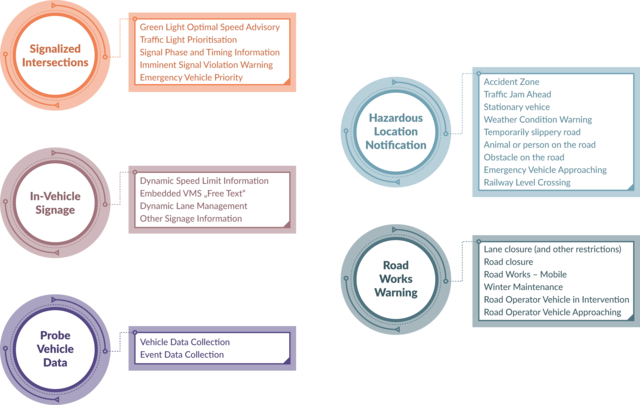
\includegraphics[width=.8\textwidth]{c-its-kolecka.png}
    \caption{C-ITS use cases \cite{2022}}
    \label{c-its-use-case}
\end{figure}

In general, the traffic safety and traffic flow improvements can be grouped based on which 
operational tasks they serve \cite{CRoads2021}: 

\begin{itemize}
    \item Provide \emph{information} to road users to improve road safety and comfort.
    \item Display \emph{regulatory boundaries} to inform road users of specific obligations, 
    restrictions or prohibitions
    \item Provide \emph{warnings} to road users about incidents ahead in their exact nature. 
\end{itemize}

To provide more insight to the design and applications of C-ITS systems, two systems are 
introduced - In-vehicle Information System and Cooperative Adaptive Cruise Control. These 
systems were selected because their operation is conditional to user engagement and are 
considered state-of-the-art application, utilizing the C-ITS technology specification. For 
those reasons, they are also relevant for the IVS-based research. 

\subsection{In-Vehicle Information System}

The In-Vehicle Information System, shortly IVIS, is a term that comprises a vast number of vehicle technology 
solutions that assist the driver either by providing information about the vehicle and the surrounding environment 
or serving as an interface to control vehicle systems. 

The integral part is the \emph{Infotainment system} (fig. \ref{ivis-interface}), which is a
video/audio interface, providing control through elements such as touch screen button panel or
voice commands.  Moreover, it integrates other vehicle technology elements, such as the CAN
interface, connectivity modules (e.g. Wi-Fi, GPS), sensors etc \cite{Saxena}. A screen panel is
an excellent medium to provide additional safety information to the driver, especially when the
gauge clusters have been replaced by an additional screen which improves the HMI aspect by
reducing the disruptive effect of checking the screen and making the displayed information more
noticeable. 

\begin{figure}[htbp]
    \centering
    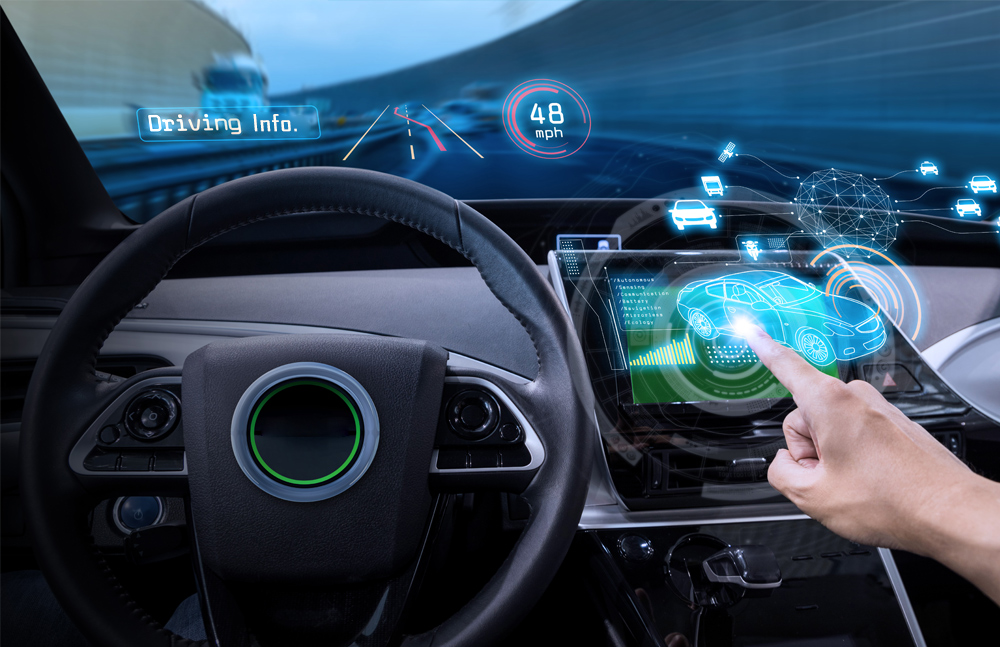
\includegraphics[width=.8\textwidth]{ivis-dashboard.jpg}
    \caption{Illustrative example of IVIS interface \cite{Saxena}}
    \label{ivis-interface}
\end{figure}

The conventional, more basic capabilities of IVIS are Heating, Ventilation, and Air
Conditioning (HVAC) control, multimedia controls, navigation support and parking assistance
(i.e. parking camera view). These systems on their own, however, aren't valuable with regard to
the thesis topic. The important feature of IVIS is the integration with the emerging C-ITS
technologies, which greatly extend the capabilities of IVIS, i.e. displaying warning and
awareness messages from the V2X interface.  This fact makes IVIS a good candidate to implement
to the IVS in the practical part, because the V2X C-ITS are a great subject for research as of
now and the distributed nature of the systems corresponds to the agent-based requirement of the
thesis topic. On top of that, the important HMI aspect of IVIS could provide great value for
future utilization in research using IVS. 

The general, a high-level solution for IVIS simulation is to provide C-ITS awareness and warning information system by 
implementing the C-ITS messaging service standard, which provides interface for broadcasting such information.
 simulating message-based communication between road users \& infrastructure and provide interface to display the 
information on the infotainment screen.

\subsection{Cooperative Adaptive Cruise Control}

The Cooperative Adaptive Cruise Control (CACC) is an extension to an already well proven ITS -
Adaptive Cruise Control.  As has been described above, this system extends the base (adaptive)
cruise control system by utilizing the V2V information broadcasted by other road users. The
system has proved to reduce the number of shock-waves by reducing oscillations that would
otherwise happen without speed information sharing and increasing capacity of the traffic
network, albeit only with higher penetration rates ($\ge 40\%$) \cite{van_Arem_2006}. Though,
regarding the introduced thesis topic requirements, the system in itself doesn't provide any
extra engagement from the driver side. 

However, another system that built upon the concept of CACC by utilizing information from the
infrastructure, namely the traffic signals, has been also recently developed this system can be
extended by sharing information about signal phasing. Consequently, adopting a speed that would
eliminate the need to stop before a red light, avoiding idle time. The system is called
\emph{Green Light Optimization Speed Advisory} (GLOSA). It uses dedicated C-ITS messages to 
share timing information among connected vehicles. Dedicated A Signal Phase and Timing (SPaT) messages 
are used to coordinate oncoming traffic speed and a Map (MAP) message to convey information 
about intersection topology. According to \cite{Pariota_2019}, the results 
of simulating deployment of this system demonstrated that even using a simple
control algorithm with the aim to avoid the stop\&go a reduction of fuel consumption
and emissions in the region of 5 to 12 \% has been observed. The study in \cite{Katsaros_2011} even 
concluded that with enough penetration, the idle (stop) time could be decreased by more than $70 \%$ 
(see fig. \ref{glosa-chart} below).

Because from the ongoing reserach and possibilities of such system, the proposed simulation architecture 
should be capable of CACC implementation - facilitating building a GLOSA traffic controller simulation
and respective interface for transmitting such information to vehicles, which will react to a received 
message conveying GLOSA timing information accordingly. 

\begin{figure}[htbp]
    \centering
    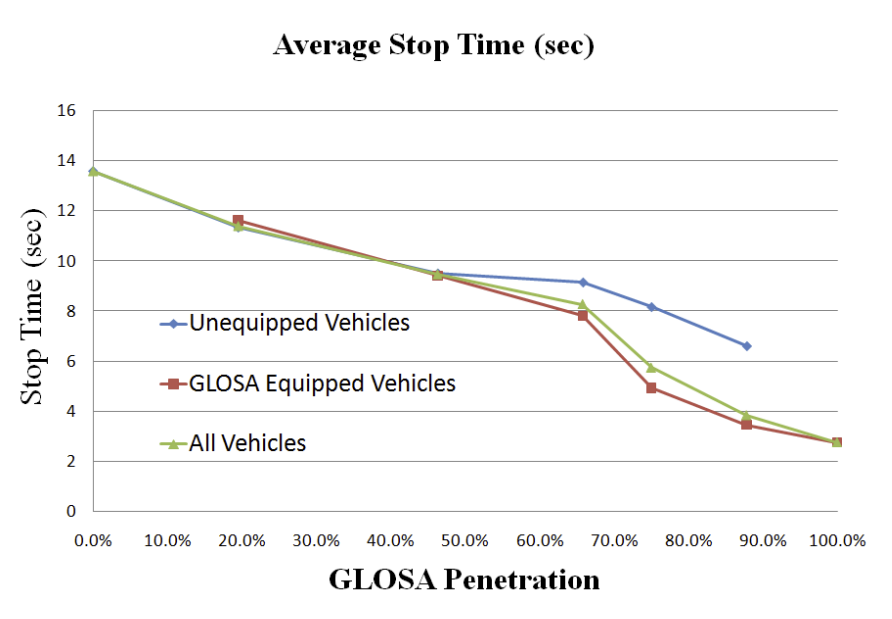
\includegraphics[width=.8\textwidth]{glosa-perf-chart.png} 
    \caption{Idle time reduction based on GLOSA penetration rate \cite{Katsaros_2011}}
    \label{glosa-chart}
\end{figure}

\subparagraph{Project C-Roads}\label{sec-croads}

In order to study the effects and refine the future deployment process of C-ITS, a project 
organized by the EU member states and road operators, called \emph{C-Roads} was established. 
The project's main objective is to harmonize C-ITS deployment activities across Europe. 
Within the C-Roads project, there have been established 5 work groups (WG), each focusing on a 
specific topic/scope regarding C-ITS objectives and priorities for research, testing and pre-
deployment of C-ITS \cite{Commision2021}. 

\begin{itemize}
    \itemspacing{0.7}
    \item WG1: Develop an EU agenda for testing
    \item WG2: Coordination and cooperation of R\&I activities
    \item WG3: Physical and digital road infrastructure
    \item WG4: Road Safety
    \item WG5: Access and exchange of data \& cyber-security
    \item WG6: Connectivity and digital infrastructure
\end{itemize}

Regarding the scope of this thesis, \emph{WG3} is the most informative segment. The focus of this group 
was, in the first place, regarding the infrastructure support for automated vehicles (SAE L4). One of 
the objectives was linking relevant physical and digital infrastructure, assessing relevance between 
them and automated vehicles, and mapping infrastructure elements to use-cases as \emph{generic driving 
tasks} (GDT):

\begin{itemize}
    \item Sensing \& Perception
    \begin{itemize}
        \itemspacing{.7}
        \item Ego localization
        \item Environmental awareness (object classification and incident detection)
        \item Enhanced perception (for limited visibility scenarios)
    \end{itemize}
    \item Planning
    \begin{itemize}
        \itemspacing{.7}
        \item (Dynamic) information and regulations
        \item Safe and appropriate navigation plans
        \item Cooperative planning
    \end{itemize}
    \item Actuation
    \begin{itemize}
        \itemspacing{.7}
        \item Motion Control
        \item Minimum Risk Manoeuvre
    \end{itemize}
\end{itemize}

It is therefore advisable to keep these General Driving Tasks in mind when thinking about the proposed framework 
features. To maximize the number of potential use-cases of the designed MAS simulation framework, 
it shall offer basic components to simulate all aforementioned GDTs, as because previous R\&I
activities have shown that the tasks above will be a fundamental part of the future C-ITS deployment.

To put these GDT use-cases into a better perspective, a mapping was created (table
(\ref{gdt-mapping})) that links the aforementioned GDTs to existing, relevant ITS solutions.
This should clear up and simplify the process of defining requirements to the proposed system,
as the new framework requirements could be easily adopted from existing system documentation of
the particular mapped ITS.



\begin{table}[htbp]
    \caption{GDT to ITS mapping}
    \renewcommand{\arraystretch}{1.3}
    \centering\begin{tabular}{lp{7em}lp{10em}} \toprule
        \multicolumn{2}{c}{GDT} & \multicolumn{2}{c}{ITS Mapping}                                                   \\ \cmidrule(r){1-2} \cmidrule(l){3-4}
        Group                   & Name                        & Type       & Description                        \\ \midrule
        \multirow{1}{3cm}
        {Sensing \& Perception} & Ego-localization            & HD Maps    & Geo-fencing                        \\
                                &                             & AD         & Self-driving algorithms            \\
                                & Environmental awareness     & IVIS       & Intersection Collision war.        \\
                                &                             &            & Emergency Vehicle war.             \\
                                &                             &            & Stationary Vehicle war.            \\
                                &                             &            & Traffic Jam war.                   \\
                                &                             &            & Traffic accident war.              \\
                                & Enhanced\newline perception & IVIS       & Overtaking war.                    \\
                                &                             &            & Intersection Collision war.        \\
                                &                             &            & VRU warning                        \\ \midrule
        Planning                & Information and regulations & CACC       & Green Light Optimal Speed Advisory \\
                                & Safe navigation plans       & Navigation & Dynamic Vehicle Routing            \\
                                & Cooperative planning        & AD         & Platooning                         \\ \midrule
        Actuation               & Motion Control              & AD         & Self-driving algorithms            \\
                                & Minimum Risk Manoeuvre      & AD         & Self-driving algorithms            \\ \midrule[1.0pt]
&&&\\
        \textbf{Legend}         &                             &            &                                    \\ \midrule
        Abbreviation            & Meaning                     &            &                                    \\ \midrule% \cmidrule(r){1-2}
        HD                      & \multicolumn{3}{l}
        {High-definition}                                                                                       \\
        AD                      & \multicolumn{3}{l}
        {Autonomous driving}                                                                                    \\
        IVIS                    & \multicolumn{3}{l}
        {In-Vehicle Information Systems}                                                                        \\
        VRU                     & \multicolumn{3}{l}
        {Vurneable Road User}                                                                                   \\
        CACC                    & \multicolumn{3}{l}
        {Cooperative Adaptive Cruise Control}                                                                   \\ \bottomrule
    \end{tabular}
    \label{gdt-mapping}
\end{table}
\clearpage
% \begin{table}[htbp]
%     \centering\begin{tabular}{ll} %\toprule
%         Abbreviation & Meaning                             \\ \midrule
%         HD           & High-definition                     \\
%         AD           & Autonomous driving                  \\
%         IVIS         & In-Vehicle Information Systems      \\
%         VRU          & Vurneable Road User                 \\
%         CACC         & Cooperative Adaptive Cruise Control \\ %\bottomrule
%     \end{tabular}
%     \caption{Legend for table \ref{gdt-mapping}}
%     \label{gdt-legend}
% \end{table}

\subsection{Conclusion}

In this section, the Intelligent Transport Systems have been introduced. This field is an
important part of traffic engineering, utilizing traffic data and mathematical modelling to
reduce congestion, improve traffic safety and reduce emissions. The main point of this section
was to discuss important features of Intelligent Transport Systems that are related to 
the topic of this thesis. The relationship between driver and ITS system, and intelligence 
distribution across ITS actors have been discussed. ITS projects relevant to the thesis topic
have been investigated, including the R\&I efforts on the EU level. The results suggested that
C-ITS systems are a current trend in research and numerous projects (e.g. C-Roads) have been
established, paving the way for the future of interconnected vehicle mobility. 

\clearpage

\end{document}